\documentclass{article}
\usepackage{graphicx}
\usepackage{subcaption}
\usepackage{hyperref}
\usepackage{float}

\title{ECNS 460 Product}
\author{Quinlin Gregg}
\date{\today}

\begin{document}

\maketitle

The goal of this product was to provide a simple way for users to quickly explore basic NFL statistics
during the 2002-2023 seasons, with insights into team and league-wide trends over that time.
(2002 was the year the Houston Texans joined the NFL, so any analysis before that would have an unequal
number of teams.) There are many factors that needs to be considered when looking though NFL data,
like team- versus game- versus league-level data and trends in the NFL. This is
why many tabs of this product have both ranked and detrended versions of the data.

The data for this product was scraped from the Pro Football Reference website in Python, exported as
a CSV file, and then was imported into R for joining, summarizing, and building the Shiny app.
I wanted to build a Shiny app in part because hosting this tool on the web would make it
more accessible as the user would not have to have R installed. However, the package for statically
hosting a Shiny app, Shiny Live, was working at the time this product was made.

ChatGPT was used to build the framework of the Shiny app, at which point it was
then modified to fit the project needs. It was also used to look up how to do various
formats in LaTeX. The challenge for this project was to build a Shiny app.
This was also my first time using LaTeX.

The app has many tabs to explore different aspects of NFL statistics. Below are some of them:

\subsection{Team Versus Team Comparisons}

This tab allows the user to compare two teams in a given statistic
over the course of the dataset. The user has 26 options which with to 
compare the teams:

\begin{itemize}
    \item Record
    \item Record Against the Spread
    \item Points Scored and Allowed, Raw and Ranked
    \item Yards Gained and Allowed, Raw and Ranked
    \item Touchdowns, Field Goals, Safeties Scored and Allowed, Raw and Ranked
    \item Punts Forced and Kicked, Raw and Ranked
\end{itemize}

The colors used match those of the teams. If the teams have colors
that are too similar (like how Denver and Cincinnati are both orange), 
then one of the teams will use a secondary fallback color
(blue for Denver and black for Cincinnati). A screenshot of this tag is in Figure 1.

\begin{figure}[H]
    \centering
    \begin{subfigure}{0.8\textwidth}
        \centering
        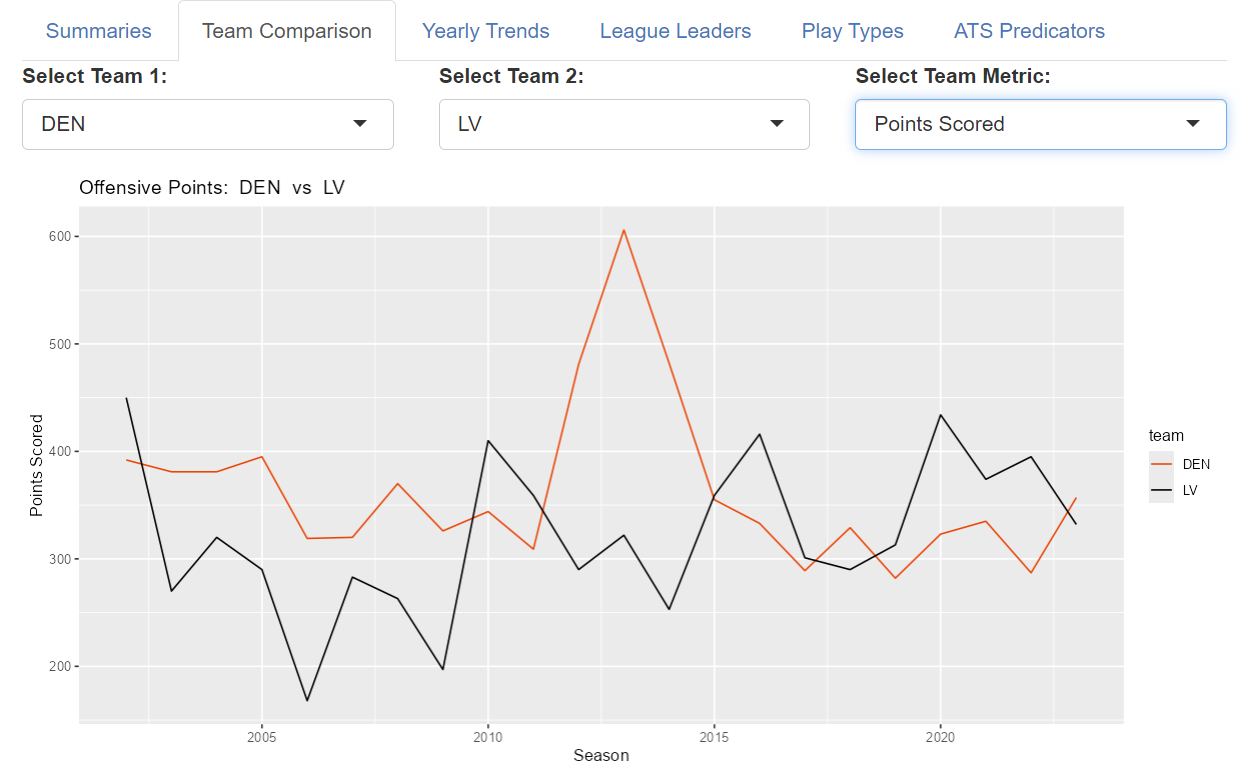
\includegraphics[width=\textwidth]{../screenshots/team-vs-team.png}
    \end{subfigure}\hfill
    \caption{Denver Broncos vs. Las Vegas Raiders Scoring Trends}
\end{figure}

\subsection{League-Wide Trends}

This section has data for cumulative league-wide statistics. This tab has
both raw and detrended versions of all statistics. 
The user can select which years they want to view out of the data.
A screenshot of this tab is in Figure 2 The options are:

\begin{itemize}
    \item Points
    \item Yards
    \item Touchdowns
    \item Field Goals
    \item Punts
\end{itemize}

\begin{figure}[H]
    \centering
    \begin{subfigure}{0.45\textwidth}
        \centering
        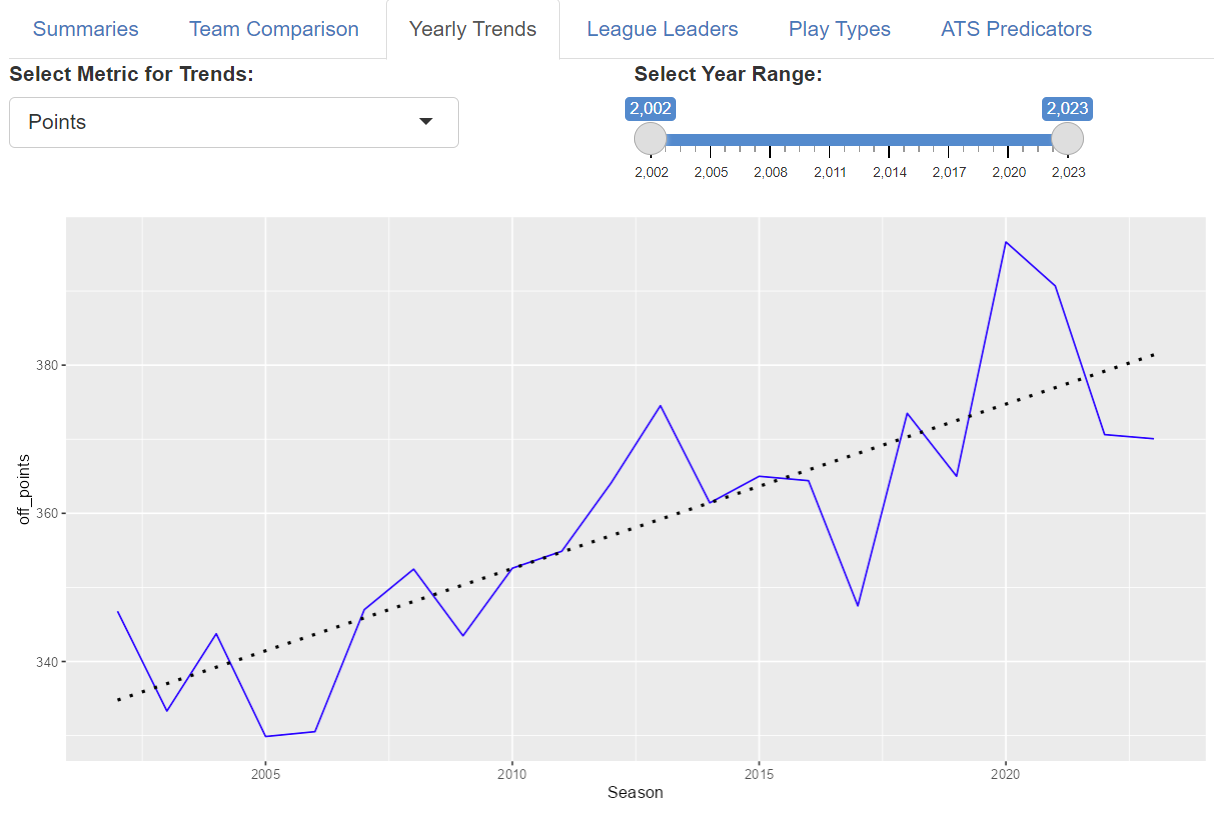
\includegraphics[width=\textwidth]{../screenshots/stat-trend.png}
    \end{subfigure}\hfill
    \begin{subfigure}{0.45\textwidth}
        \centering
        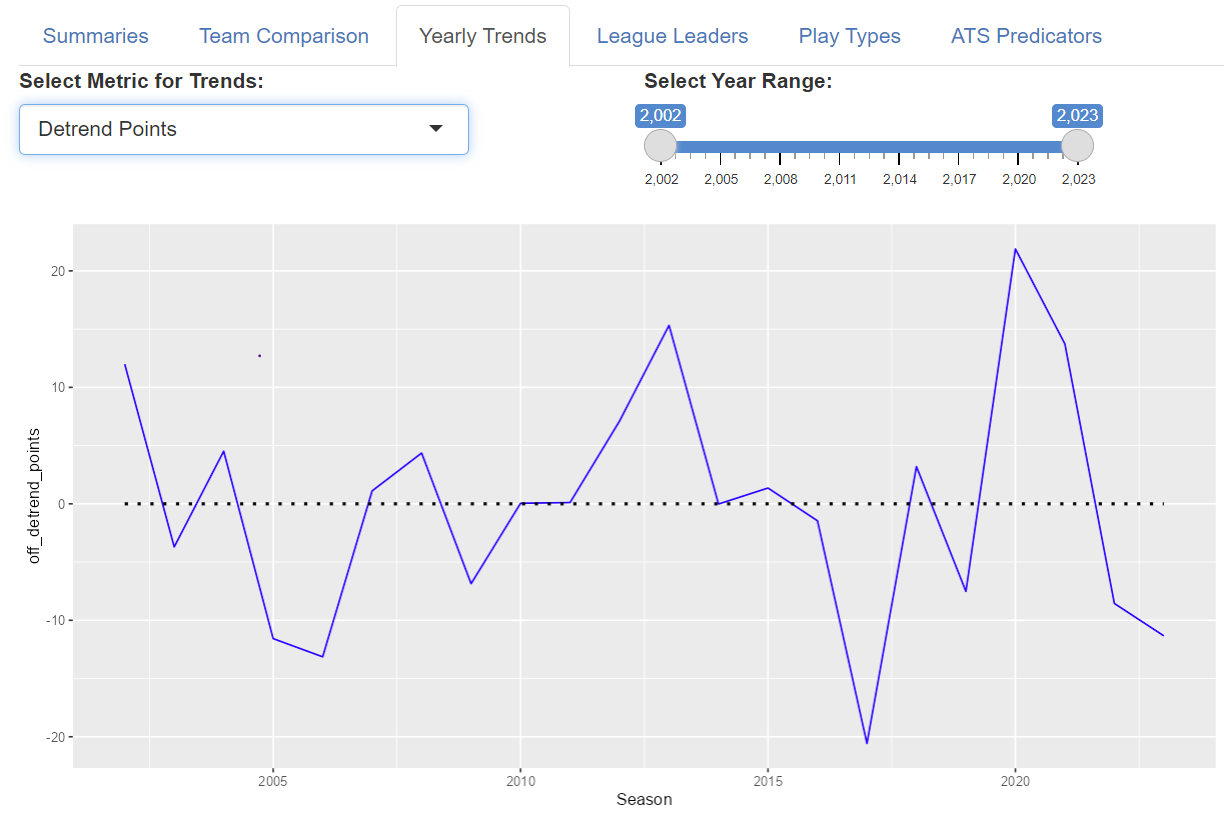
\includegraphics[width=\textwidth]{../screenshots/stat-detrend.png}
    \end{subfigure}\hfill
    \caption{Plots showing total points scored and detrend points scored}
\end{figure}

\subsection{Team Totals}

This tab allows the user to view how each team has done cumulatively
over this period in a ranked view. The options here are the same
as in the team versus team comparisons.

\begin{figure}[H]
    \centering
    \begin{subfigure}{0.8\textwidth}
        \centering
        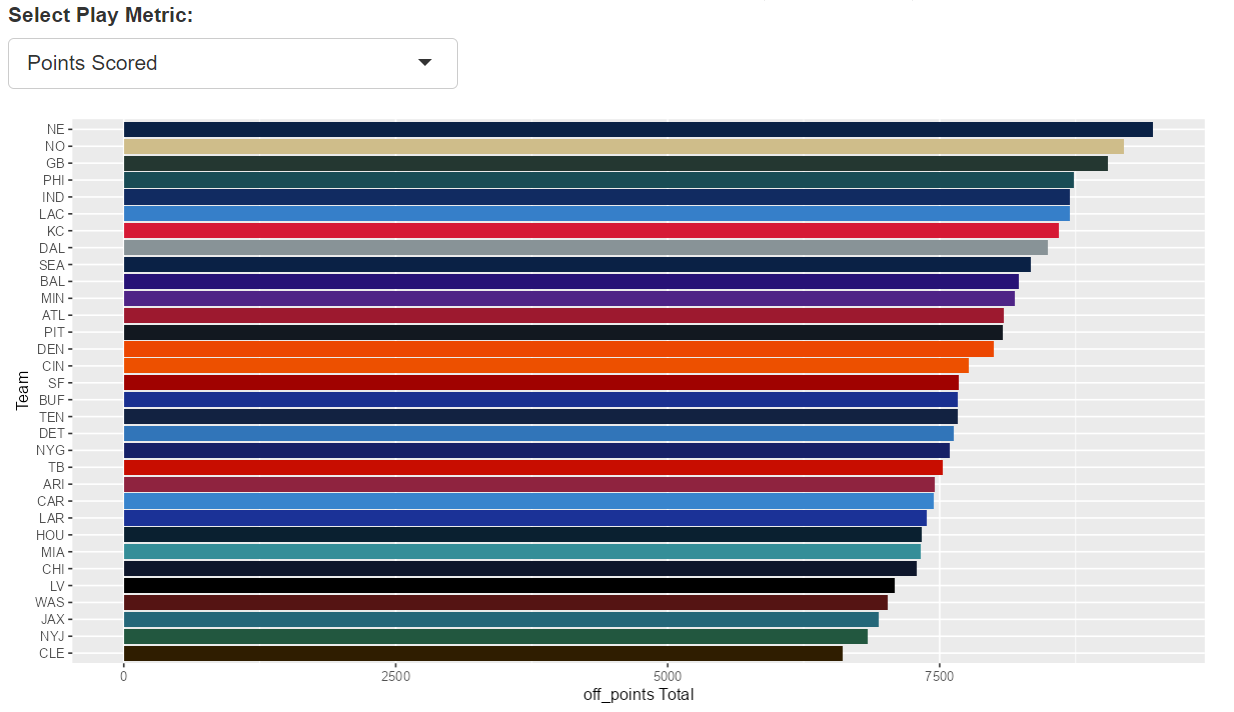
\includegraphics[width=\textwidth]{../screenshots/team-totals.png}
    \end{subfigure}\hfill
    \caption{The teams ranked by total points scored from 2002-2023}
\end{figure}

\subsection{Record Predictors}

This tab allows the user to investigate how various statistics correlate
to record and record against the spread. The choices for statistics are the
same as in the team versus team tab. It displays a scatterplot of the variables, 
a line of best fit and its coefficients, and the $R^{2}$ between the variables.
A screenshot is in Figure 4.

\begin{figure}[H]
    \centering
    \begin{subfigure}{0.45\textwidth}
        \centering
        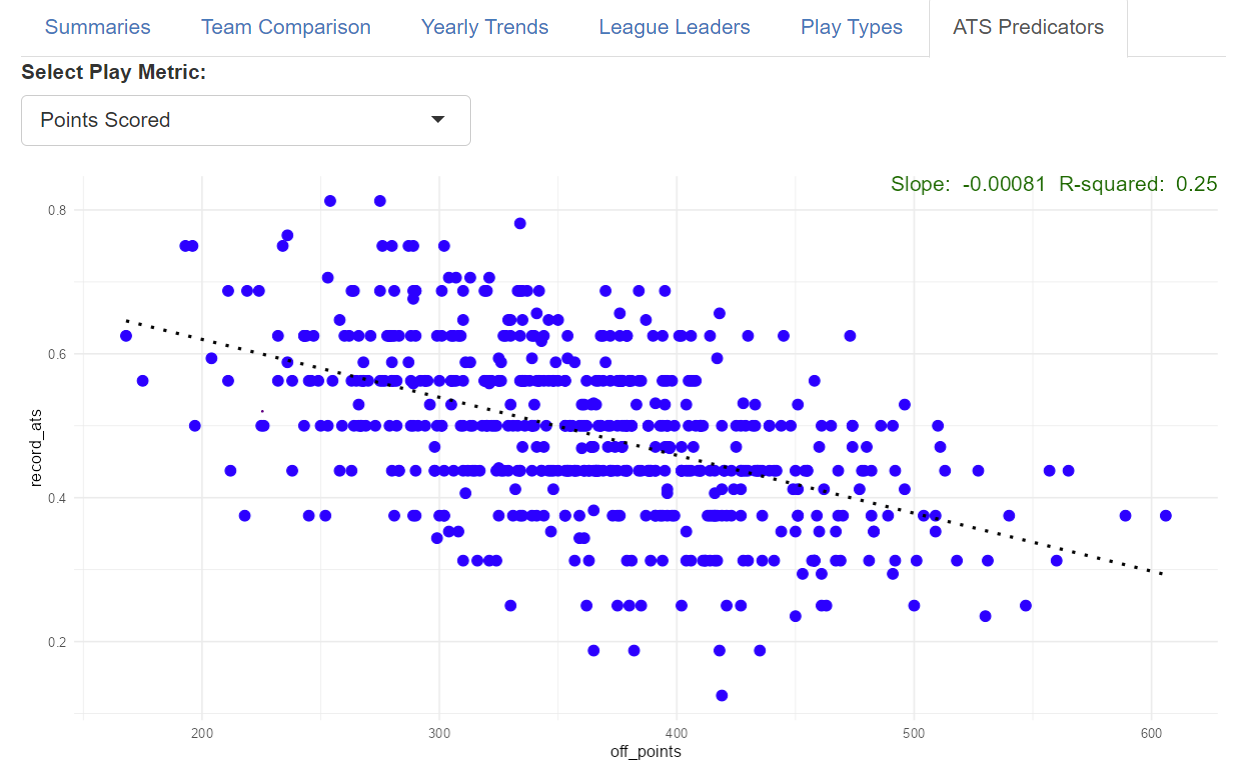
\includegraphics[width=\textwidth]{../screenshots/ats-trend.png}
    \end{subfigure}\hfill
    \begin{subfigure}{0.45\textwidth}
        \centering
        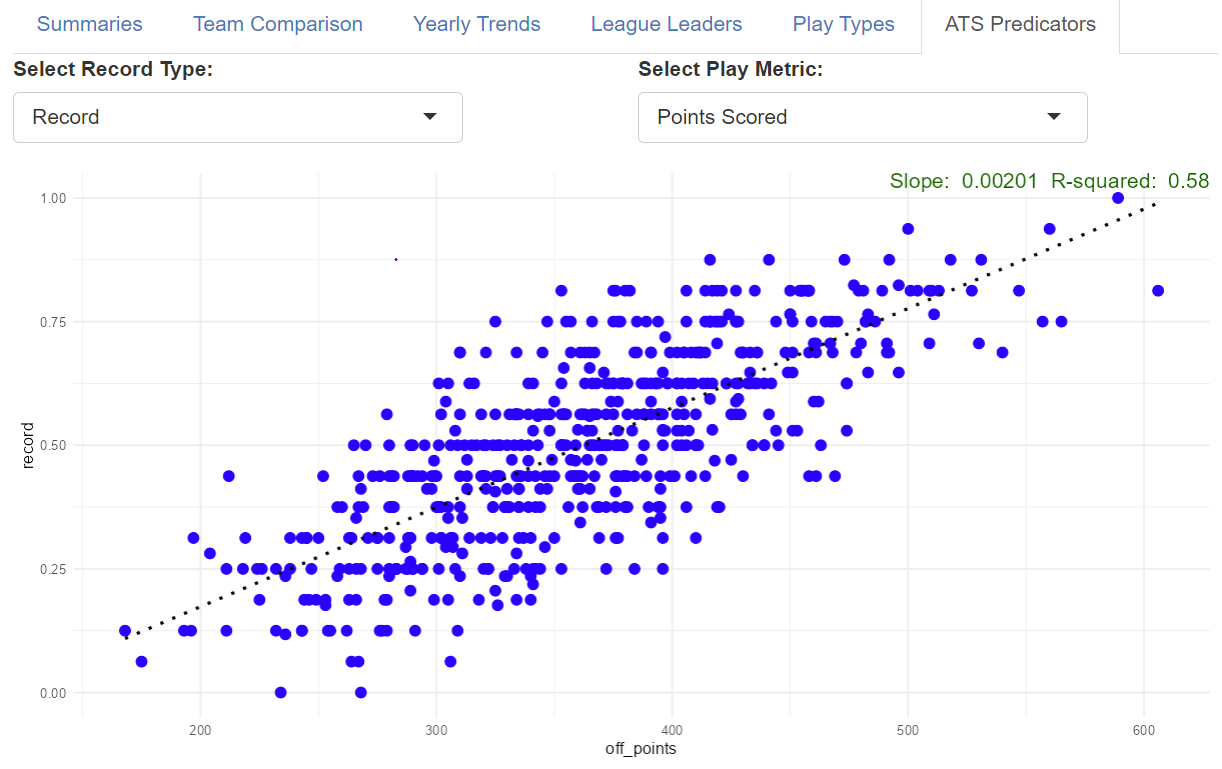
\includegraphics[width=\textwidth]{../screenshots/record-trend.png}
    \end{subfigure}\hfill
    \caption{Points scored versus record (left) and record against the spread (right)}
\end{figure}

\end{document}
